\documentclass[11pt,aspectratio=43,ignorenonframetext,t]{beamer}
% Uses fontspec - assumes compiled with LuaLaTeX or similar
% The above \documentclass is for making slides. If making handouts use:
%\documentclass[11pt,a4paper]{article} 
%\usepackage{beamerarticle}
%\setjobnamebeamerversion{main.beamer}

% See https://github.com/CASSON-LAB/uom_beamer_template
% for details on license, further useage information and similar
%%%%%%%%%%%%%%%%%% DOCUMENT SETUP %%%%%%%%%%%%%%%%%%

% Presentation settings
\mode<presentation>{
  \usetheme[framenumber,titleframestart=1]{UoM_alex}
  \usefonttheme{professionalfonts} % using non standard fonts for beamer
  \usefonttheme{serif}             % set font to Arial
  \usepackage{fontspec}
  \setmainfont[Ligatures=TeX]{Arial}
}

% Handout settings
\mode<article>{
  \usepackage{fullpage}                  % use full page
  \usepackage{fontspec}                  % set font to Arial
    \setmainfont[Ligatures=TeX]{Arial}
  \setlength{\parskip}{1.5\baselineskip} % correct beamer line spacings
  \setlength{\parindent}{0cm}
  \usepackage{enumitem}
    \setlist[itemize]{topsep=0pt}
  \definecolor{uomlinkblue}{HTML}{0071BC}
}


% Packages

% Configurando layout para mostrar codigos C++
\usepackage{listings}
\lstset{
  language=HTML,
  basicstyle=\ttfamily\small, 
  keywordstyle=\color{blue}, 
  stringstyle=\color{red}, 
  commentstyle=\color{red}, 
  extendedchars=true, 
  showspaces=false, 
  showstringspaces=false, 
  numbers=left,
  numberstyle=\tiny,
  breaklines=true, 
  backgroundcolor=\color{green!10},
  breakautoindent=true, 
  captionpos=b,
  xleftmargin=0pt,
}

\usepackage{graphicx}  % for graphics files
  \graphicspath{ {./fig/aula6} }
\usepackage{amsmath}   % assumes amsmath package installed
  \allowdisplaybreaks[1] % allow eqnarrays to break across pages
\usepackage{amssymb}   % assumes amsmath package installed 
\usepackage{hyperref} % add hyperlinks to document. Settings are for accessiblity
  \hypersetup{
    colorlinks=true,
    linkcolor=uomlinkblue,
    filecolor=uomlinkblue,      
    urlcolor=uomlinkblue,
	pdflang={en-GB},
}
\usepackage[document]{ragged2e} % left aligned text for accessibility
% experimental - does fundamentally work, if with quite a bit of effort
%\usepackage{axessibility} % LaTeX readable equations for accessibility
%  \tagpdfsetup{tabsorder=structure,uncompress,activate-all,interwordspace=true}
%  \pdfextension catalog{/Lang (en-GB)}
%  \RequirePackage{luacode}
%  \directlua{require("axessibility.lua")}
\usepackage{unicode-math} % unicode maths for accessibility
\usepackage{pdfcomment} % for alt text for accessibility
\usepackage{rotating}  % allow portrait figures and tables
\usepackage{subfigure} % allow matrices of figures
\usepackage{float}     % allows H option on floats to force here placement
\usepackage{multirow}  % allows merging of rows in tables
\usepackage{tabularx}  % allows fixed width tables
\usepackage{ctable}    % modifies \hline for use in table
\usepackage{bm}        % allow bold fonts in equations
\usepackage{pgf}       % allow graphics manipulation
\usepackage{media9}    % allow interactive flash files to be embedded
  \addmediapath{../media}
\usepackage{etoolbox}
  \makeatletter \preto{\@verbatim}{\topsep=0pt \partopsep=0pt} \makeatother  
  
% Custom commands
\newcommand{\matlab}{\emph{\sc{Matlab}}}
\newcommand{\maple}{\emph{\sc{Maple}}}
\newcommand{\simulink}{\emph{\sc{Simulink}}}
\newcommand{\dc}{d.c.}
\newcommand{\ac}{a.c.}
\newcommand{\rms}{RMS}
\newcommand{\wgn}{{\tt wgn}}
\newcommand{\sus}[1]{$^{\mbox{\scriptsize #1}}$}
\newcommand{\sub}[1]{$_{\mbox{\scriptsize #1}}$}
\newcommand{\chap}[1]{Chapter~\ref{#1}}
\newcommand{\sect}[1]{Section~\ref{#1}}
\newcommand{\fig}[1]{Fig.~\ref{#1}}
\newcommand{\tab}[1]{Table~\ref{#1}}
\newcommand{\equ}[1]{(\ref{#1})}
\newcommand{\appx}[1]{Appendix~\ref{#1}}
\newcommand{\degree}{\ensuremath{^\circ}}
\newcommand{\Vrms}{Vrms}
\newcommand{\Vpp}{V\sub{pp}}
\newcommand{\otoprule}{\midrule[\heavyrulewidth]}         
\newcolumntype{Z}{>{\centering\arraybackslash}X}  % tabularx centered columns 
\makeatletter \DeclareRobustCommand{\em}{\@nomath\em \if b\expandafter\@car\f@series\@nil \normalfont \else \bfseries \fi} \makeatother
\newcounter{example_number} % keep track of the example questions



%%%%%%%%%%%%%%%%%% FRONT MATTER %%%%%%%%%%%%%%%%%%
\title{Análise Orientada a objetos}
\subtitle{Aula 7}
\author{Prof. Me. Juliana Costa-Silva}

\begin{document}

\maketitle
%%%%%%%%%%%%%%%%%% TITLE SLIDE %%%%%%%%%%%%%%%%%%
\mode<presentation>{ \frame{\titlepage \label{slide:a}}} 
%\begin{figure}[!ht] 
%\fbox{\includeslide[width=\textwidth]{slide:a}} \end{figure}

%------------------------------------------------------------------------
% \section{Introdução}
 \mode<presentation>{ 
 \begin{frame}{Na última aula...}
 \begin{itemize}
  \item Objetos;
  \item Classes;
  \end{itemize}
\end{frame}
}
%-------------------------------------------------------------------------
 \mode<presentation>{ 
\begin{frame}
\frametitle{Na aula de hoje...} 
\tableofcontents 
\end{frame}
}
%----------------------------------------------------------------------------
\section{static}
 \mode<presentation>{ 
\begin{frame}{Static}
  \begin{itemize}
    \item Atributos e métodos estáticos são compartilhados por todos os objetos 
criados a partir daquela classe.
    \item Existe apenas uma única cópia do método e/ ou atributo que esta 
associada com a classe e não com alguma instância criada da classe (objetos).
  \end{itemize}
  \begin{columns}
    \begin{column}{0.4\textwidth}
      \begin{block}{Atributos e métodos estáticos}
      pertencem à classe
     \end{block}

    \end{column}
    \begin{column}{0.4\textwidth}
     \begin{block}{Atributos e métodos não-estáticos}
      pertecem ao objeto
     \end{block}
    \end{column}
  \end{columns}

\end{frame}
}
%----------------------------------------------------------------------------
 \mode<presentation>{ 
\begin{frame}{static}
  Restrições:
    \begin{itemize}
      \item um método estático, \textbf{\textcolor{blue}{NÃO}} pode acessar 
variáveis de instância;
       \item um método estático, \textbf{\textcolor{blue}{NÃO}} pode se 
referenciar a métodos de instância.
    \end{itemize}
\end{frame}
}
%----------------------------------------------------------------------------
 \mode<presentation>{ 
\begin{frame}{static}

  \small{ 
\lstinputlisting[linerange={3-8}]{./cod/Estatico.java}
  }
\end{frame}
}
%----------------------------------------------------------------------------
 \mode<presentation>{ 
\begin{frame}{static}
   \small{\lstinputlisting[linerange={3-15}]{./cod/TestaEstatico.java}}
\end{frame}
}
%--------------------------------------------e--------------------------------
%----------------------------------------------------------------------
\section{Atividade}
 \mode<presentation>{ 
\begin{frame}{Atividade}
  \begin{enumerate}
   \item Modele um funcionário. Ele deve ter o nome do funcionário, o 
departamento onde trabalha, seu salário (double), a data de entrada no banco 
(String), seu RG (String) e um valor booleano que indique se o funcionário está na empresa no momento ou se já foi embora. Você deve criar alguns métodos de  acordo com sua necessidade. 
    \item Além deles, crie um método bonifica que aumenta o salário do 
funcionário de acordo com o parâmetro passado como argumento. Crie, também, um 
método demite , que não recebe parâmetro algum, só modifica o valor booleano 
indicando que o funcionário não trabalha mais aqui.
  \end{enumerate}
\end{frame}
}
%--------------------------------------------------------
 \mode<presentation>{ 
\begin{frame}{Atividade}
  \begin{enumerate}
   \item Transforme o modelo em uma classe Java. Teste-a, usando uma outra 
classe que tenha o main. Você deve criar a classe do funcionário chamada  
Funcionario , e a classe de teste você pode nomear como quiser. A de teste deve 
possuir o método main. Um esboço das classes:
  \end{enumerate}
  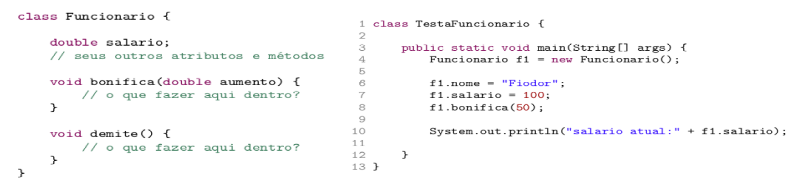
\includegraphics[height=0.3\paperheight]{classes_AEP1.png} \\
\end{frame}
}
%-----------------------------------------------------------------------
%----------------------------------------------------------------------------
\section{Classe Time1}
 \mode<presentation>{ 
\begin{frame}{Time1.java}
\small{ 
\lstinputlisting[linerange={2-12}]{./cod/Time1.java}}
\end{frame}
}
%----------------------------------------------------------------------------
 \mode<presentation>{ 
\begin{frame}{Time1.java - Parte II}
\small{ 
\lstinputlisting[linerange={13-24}]{./cod/Time1.java}}
\end{frame}
}
%----------------------------------------------------------------------------
 \mode<presentation>{ 
\begin{frame}{Entendendo...}
O que fizemos nesse trecho?
 \small{ 
\lstinputlisting[linerange={2-5}]{./cod/Time1.java}}
\end{frame}
}
%----------------------------------------------------------------------------
 \mode<presentation>{ 
\begin{frame}{Entendendo...}
O que faz esse método?
 \small{ 
\lstinputlisting[linerange={7-11}]{./cod/Time1.java}}
\end{frame}
}
%----------------------------------------------------------------------------
 \mode<presentation>{ 
\begin{frame}{Entendendo...}
O que não entendemos nos métodos abaixo?
 \small{ 
\lstinputlisting[linerange={13-15}]{./cod/Time1.java}}

 \small{ 
\lstinputlisting[linerange={17-22}]{./cod/Time1.java}}
Anote as explicações, como comentários no código
\end{frame}
}
%----------------------------------------------------------------------------
 \mode<presentation>{ 
\begin{frame}{Testando...}
Crie uma classe Time1Test e declare um método main() nessa classe. E faça 
testes!
 \small{ 
\lstinputlisting[linerange={2-9}]{./cod/Time1Test.java}}
Não se esqueça de fechar as chaves da classe e da main()!!
\end{frame}
}
%----------------------------------------------------------------------------
 \mode<presentation>{ 
\begin{frame}{Testando II}
 \small{ 
\lstinputlisting[linerange={11-17}]{./cod/Time1Test.java}}
 
\end{frame}
}
%----------------------------------------------------------------------
\section{Controle de acesso}
 \mode<presentation>{ 
\begin{frame}{Controle de acesso}
Altere o valor dos atributos na main() da classe TimeTest.java
 \small{ 
\lstinputlisting[linerange={19-19}]{./cod/Time1Test.java}}

\textcolor{red}{Exception in thread ``main'' java.lang.RuntimeException: 
  Uncompilable source code \- hora has private access in Time1Test}\\

\vspace{0.3cm}
\begin{block}{Como editar os valores?}
 Os valores serão editados, somente utilizando o construtor da classe, ou com a 
chamada dos métodos que fazem a  edição, nesse caso método \underline{setTime}.
\\
 Isso se deve ao operador de visibilidade \textcolor{purple}{private}.
\end{block}
\end{frame}
}
%----------------------------------------------------------------------
\section{Construtor}
 \mode<presentation>{ 
\begin{frame}{Construtor de classe}
E se houver a necessidade de inicializarmos um objeto com um valores, sem 
utilizar um método para alterar os valores de atributos?\\
% 
% Declare um CONSTRUTOR para a classe:
%  \small{ 
% \lstinputlisting[linerange={1-11}]{./codigo/Aula11/src/Time2.java}}
\end{frame}
}
%----------------------------------------------------------------------
 \mode<presentation>{ 
\begin{frame}{Construtor de classe}
  Declare um CONSTRUTOR para a classe:
 \small{ 
\lstinputlisting[linerange={1-11}]{./cod/Time2.java}}
  
Utilizando o CONSTRUTOR da classe Time2:
 \small{ 
\lstinputlisting[linerange={3-3}]{./cod/Time2Test.java}}
\end{frame}
}
%----------------------------------------------------------------------
 \mode<presentation>{ 
\begin{frame}{Construtor de classe}
  Construtor é o método que instancia um objeto, quando utilizamos \textit{new} 
String(), estamos utilizando o construtor da classe String.\\
\vspace{0.5cm}

\begin{itemize}
 \item Construtores possuem o mesmo nome da classe;
  \item É indicado que toda classe possua ao menos um construtor;
  \item O construtor não precisa necessariamente inicializar todos os 
atributos da classe.
   \item Uma classe pode ter vários Construtores.
\end{itemize}

\end{frame}
}
%----------------------------------------------------------------------
\section{Sobrecarga de Construtor}
 \mode<presentation>{ 
\begin{frame}{Construtor de classe}
  Vejamos como criar vários Construtores em uma classe
 \small{ 
\lstinputlisting[linerange={13-20}]{./cod/Time2.java}}
\end{frame}
}
%----------------------------------------------------------------------
 \mode<presentation>{ 
\begin{frame}{Construtor de classe}
  Vejamos como \underline{utilizar} vários Construtores em uma classe
 \small{ 
\lstinputlisting[linerange={3-6}]{./cod/Time2Test.java}}
\end{frame}
}
%----------------------------------------------------------------------
\section{Get e Set}
 \mode<presentation>{ 
\begin{frame}{Manipulando atributos}
  E se precisarmos alterar apenas o valor do atributo hora, sem editar os 
outros valores?\\

 \small{ 
\lstinputlisting[linerange={22-29}]{./cod/Time2.java}}
  Para manipular valores de atributos, a classe deve possuir métodos get e set 
para cada um de seus atributos.\\

\textcolor{red}{Podemos receber valores de hora sem validar?}\\
Desenvolva os métodos get e set da classe Time2, com validação.
\end{frame}
}
%----------------------------------------------------------------------
\section{Atividade}
 \mode<presentation>{ 
 \begin{frame}{Atividade}
  \begin{enumerate}
   \item Como ficam os métodos setTime, toString e toUniversalString na classe 
Time2? Implemente-os.
    \item Teste os métodos.
    \item Na main, utilize dois objetos Time2, guarde dois horários recebidos 
pelo usuário e retorne a diferença do valor de horas e minutos entre os dois 
objetos.
    \item Crie um método na classe Time2 que receba um valor inteiro e uma 
String. O método deve adicionar o valor inteiro recebido por parâmetro ao 
atributo recebido como String ``hora'', ``minuto'' ou ``segundo''.
  \end{enumerate}
\end{frame}
}
% %--------------------------------------------------------
% \mode<presentation>{ \begin{frame}{Atividade - AEP I}
%   \begin{enumerate}
%    \item Transforme o modelo em uma classe Java. Teste-a, usando uma outra 
% classe que tenha o main. Você deve criar a classe do funcionário chamada  
% Funcionario , e a classe de teste você pode nomear como quiser. A de teste deve 
% possuir o método main. Um esboço das classes:
%   \end{enumerate}
%   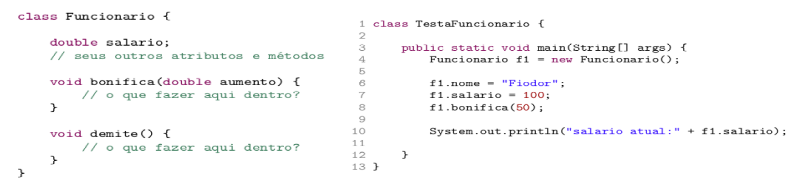
\includegraphics[height=0.3\paperheight]{classes_AEP1.png} \\
% \end{frame}

%----------------------------------------------------------------------------
\section{Classes}
 \mode<presentation>{ 
\begin{frame}{Conta.java}
  E se quisermos colocar um valor padrão (\textit{default}) para nossos 
atributos?\\
\begin{center}
  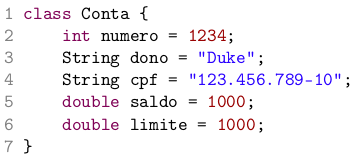
\includegraphics[height=0.3\paperheight]{conta2.png} \\
 \end{center}
  Nesse caso os atributos de um objeto são populados com os valores 
definidos na declaração dos atributos, e ao criarmos um objeto ele já esta 
populado.
\end{frame}
}
%----------------------------------------------------------------------------
 \mode<presentation>{ 
\begin{frame}{Cliente.java e Conta.java}
  Um atributo também pode ser uma referência para outra classe.\\
  Vejamos a classe cliente:
  \begin{columns}
    \begin{column}{0.4\textwidth}
      \begin{center}
	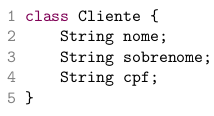
\includegraphics[height=0.25\paperheight]{cliente.png} \\
      \end{center}
   \end{column}
   \begin{column}{0.4\textwidth}
      \begin{center}
	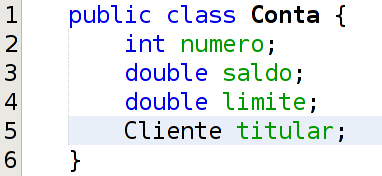
\includegraphics[height=0.2\paperheight]{contaCliente.png} \\
      \end{center}
   \end{column}

  \end{columns}

\end{frame}
}
%----------------------------------------------------------------------------
 \mode<presentation>{ 
\begin{frame}{Teste.java}
  \begin{center}
      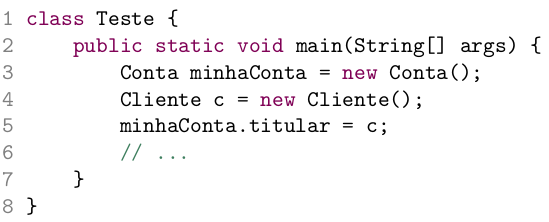
\includegraphics[height=0.35\paperheight]{contaClienteMain.png} \\
  \end{center}
  
  Aqui, simplesmente houve uma atribuição. \\ 
  O valor da variável c é copiado para  o atributo titular do objeto ao qual 
minhaConta se refere. \\ 
Em outras palavras, minhaConta agora tem uma referência ao mesmo Cliente que c 
se refere, e pode ser acessado através de minhaConta.titular.  
\end{frame}
}
%----------------------------------------------------------------------------
 \mode<presentation>{ 
\begin{frame}{Funcionario.java}
Vejamos a classe que registra os funcionários do banco.
 \small{ 
\lstinputlisting[linerange={2-7}]{./cod/Banco/Funcionario.java}}
 Crie os métodos get e set para cada atributo da classe.
\end{frame}
}
%----------------------------------------------------------------------------
 \mode<presentation>{ 
\begin{frame}{Gerente.java}
Vejamos a classe que registra os Gerentes do banco.
 \small{ 
\lstinputlisting[linerange={3-20}]{./cod/Banco/Gerente.java}}

Repetimos alguns trechos de código?
\end{frame}
}
%----------------------------------------------------------------------------
 \mode<presentation>{ 
\begin{frame}{Pensando...}
\begin{itemize}
 \item E se tivéssemos mais algum tipo de funcionário?
  \item Se for necessário guardar mais alguma informação sobre todos os 
funcionários? Teríamos que editar todas as classes (Funcionario, Gerente, 
Tipo3...)
   \item Existe uma maneira de relacionarmos uma classe de tal maneira que 
  uma delas \textbf{herda} tudo que a outra tem. 
   \item Isto é uma relação de \underline{classe mãe} e \underline{classe filha}. 
    \item No nosso caso, gostaríamos de fazer com que o Gerente tivesse tudo que um Funcionario tem, gostaríamos que ela fosse uma extensão de  
Funcionario. 
 \item Fazemos isto através da palavra chave \textit{extends}.
\end{itemize}

\end{frame}
}
%----------------------------------------------------------------------------
\section{Herança}
 \mode<presentation>{ 
 \begin{frame}{Herança}
 \small{ 
\lstinputlisting[linerange={1-13}]{./cod/Banco/Gerente.java}}
\end{frame}
}
%----------------------------------------------------------------------
 \mode<presentation>{ 
 \begin{frame}{Utilizando a nova classe Gerente}
 \small{ 
\lstinputlisting[linerange={2-8}]{./cod/Banco/TestaGerente.java}}
\vspace{0.3cm}
\begin{block}{Super e Sub classe}
 A nomenclatura mais encontrada é que Funcionario é a 
superclasse de Gerente, e Gerente é a subclasse de Funcionario. Dizemos também 
que todo Gerente é um Funcionário.
\end{block}

\end{frame}
}
%----------------------------------------------------------------------
\section{Reescrita de métodos}
 \mode<presentation>{ 
 \begin{frame}{Funcionario.java}
Como controlar a bonificação dos funcionários?\\

Vamos criar o método bonificação:
\small{ 
\lstinputlisting[linerange={8-10}]{./cod/Banco/Funcionario.java}}

Porém queremos que Gerentes tenham uma bonificação de 15\% e os outros 
funcionários uma bonificação de 10\%.

\textbf{Teste a bonificação de Gerente e Funcionário.}
\end{frame}
}
%----------------------------------------------------------------------
 \mode<presentation>{
\begin{frame}{Reescrita de métodos}
 Na classe Gerente.java reescreva o método getBonificacao().
  \small{ 
\lstinputlisting[linerange={15-16}]{./cod/Banco/Gerente.java}}
Execute o teste novamente...
\end{frame}
}
%----------------------------------------------------------------------
\section{Atividade}
 \mode<presentation>{
\begin{frame}{Atividade}
  \begin{enumerate}
   \item Crie uma classe Conta, que possua um saldo, e os métodos para pegar 
saldo, depositar, e sacar.
    \item Crie os métodos get e set para cada atributo.
    \item Adicione um método na classe Conta, que atualiza o saldo da conta de 
acordo com uma taxa percentual fornecida.
    \item Crie duas subclasses da classe Conta : ContaCorrente e ContaPoupanca. Ambas terão o método atualiza reescrito: A ContaCorrente deve atualizar-se com o dobro da taxa e a ContaPoupanca deve atualizar-se com o triplo da taxa.
    \item Além disso, a ContaCorrente deve reescrever o método deposita, afim de retirar uma taxa bancária de dez centavos de cada depósito.
    \item Crie uma classe com método main e instancie essas classes, atualize-as e veja o resultado.
  \end{enumerate}
\end{frame}
}
%----------------------------------------------------------------------
 \mode<presentation>{
\begin{frame}{Atividade - PARCIAL}
\small
  \begin{itemize}
   \item \textbf{1.} Faça com que sua classe Pessoa possa receber, opcionalmente, o nome do titular durante a criação do objeto. Envie o código Java como resposta.
   \item \textbf{2.} Atualize a suas classes que acessam e modificam atributos de uma Pessoa para utilizar os getters e setters recém-criados. Indique o que foi alterado, em qual arquivo e por que.
   \item \textbf{3.} O que é necessário fazer para garantirmos que os atributos de uma classe não sejam acessados de forma direta em outra classe a qual não seja a própria classe? Descreva a sua solução e Justifique.
   \item \textbf{4.} Imagine que tenhamos a classe PessoaFisica a qual tem um CPF como atributo. Como garantir que alguma pessoa física tenha CPF inválido e tampouco seja criada uma PessoaFisica sem CPF inicial? (Suponha que já exista um algoritmo de validação de CPF: este deve passar por um método  valida(String x)....)
   \end{itemize}
\end{frame}
}

%----------------------------------------------------------------------
 \mode<presentation>{
\begin{frame}{Atividade - PARCIAL}
\small
  \begin{itemize}
   \item \textbf{5.} Após deixar os atributos da classe Pessoa (atributos: cpf, nome, nascimento) com acesso restrito (privado), tente criar uma Pessoa na classe TestaPessoa dentro do main e modificar ou ler os atributos da Pessoa criada. O que acontece? Crie apenas os getters e setters necessários na sua classe Pessoa. Pense sempre se é preciso criar cada um deles. *Não copie e cole! Aproveite para praticar a sintaxe.
   \item \textbf{6.} Adicione um atributo, na classe Pessoa de tipo int, que se chama identificador. Este deve ter um valor único para cada instância do tipo Pessoa. A primeira Pessoa instanciada tem identificador 1, a segunda, 2, e assim por diante. Você deve utilizar os recursos aprendidos aqui na resolução desse problema.
   \end{itemize}
\end{frame}
}
% %--------------------------------------------------------
% \mode<presentation>{ 
% \begin{frame}{Atividade - AEP I}
%   \begin{enumerate}
%    \item Transforme o modelo em uma classe Java. Teste-a, usando uma outra 
% classe que tenha o main. Você deve criar a classe do funcionário chamada  
% Funcionario , e a classe de teste você pode nomear como quiser. A de teste deve 
% possuir o método main. Um esboço das classes:
%   \end{enumerate}
%   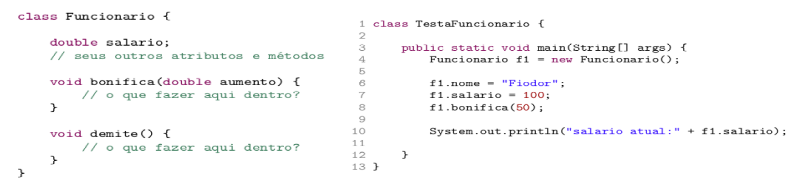
\includegraphics[height=0.3\paperheight]{classes_AEP1.png} \\
% \end{frame}
%}
%-----------------------------------------------------------------------
\section{Leitura recomendada}
 \mode<presentation>{
\begin{frame}{Leitura complementar}
 Para mais informações sobre JAVA, leia:\\
 \begin{columns}
   \begin{column}{0.4\textwidth}
     Java: Como programar\\
     Capítulo 3:\\ 
      \cite{deitel2010java}
   \end{column}
   \begin{column}{0.3\textwidth}
    \begin{center}
  
\includegraphics[height=0.5\paperheight]{fig/aula1/deitel2017java.png} \\
 \end{center}
   \end{column}
 \end{columns}
\end{frame}
}
%----------------------------------------------------------------------------------------------------------------------
 
 \mode<presentation>{\begin{frame}{Referências}%[allowframebreaks]
 \small
 \begin{center}
 	\bibliographystyle{apalike}
	 \bibliography{ref_aula_progI}
 \end{center}
 \end{frame}}

\begin{figure}[!ht] \fbox{\includeslide[width=\textwidth]{slide:z}} \end{figure}
Text for notes goes here. 
\begin{itemize}
  \item List 1. 
  \item List 2. 
\end{itemize}


%%%%%%%%%%%%%%%%%% END MATTER %%%%%%%%%%%%%%%%%%
\end{document}